% Helsinki Logic Group talk, 11 November 2026 (Moloch theme, serif).
% Its text is kept in talk_hlg_111126_text.md, its slide notes in
% talk_hlg_111126_notes.md, and the overview diagram in
% talk_hlg_111126_diagram_full.tex and talk_hlg_111126_diagram_partial.tex.
%
% Build from this folder (the PDF lands here; auxiliary files go to the
% gitignored communication_drafts/build/ folder). Build the two diagrams first:
%   latexmk -pdf -auxdir=../build talk_hlg_111126_diagram_full.tex
%   latexmk -pdf -auxdir=../build talk_hlg_111126_diagram_partial.tex
%   latexmk -pdf -auxdir=../build talk_hlg_111126.tex
%
% Reveal pattern for a slide: step 1 is the paragraph as is. From step 2, each click
% marks one word with \revealedword<n-> and shows its line with \item<n->, which
% repeats the word with \markedword. Each concept has its own colour, defined in
% the preamble.

\documentclass[aspectratio=169,10pt]{beamer}

\usetheme{moloch}
% For the two small diagrams (Pitch, Process): arrow tips, and boxes fitted around
% a group of nodes.
\usetikzlibrary{arrows.meta, fit}
\usepackage{mathpazo}
\usefonttheme{serif}
% New dependency: ulem, for the strikethrough on the Science slide. normalem keeps
% \emph as italics.
\usepackage[normalem]{ulem}
% New dependency: multimedia, for the video on the rising sea. pdfpc plays it on a
% click (it does not support autoplay); the .mp4 must sit next to the PDF.
\usepackage{multimedia}
\setbeamersize{text margin left=1.4em, text margin right=1.4em}
\setbeamertemplate{navigation symbols}{}
\setbeamertemplate{page number in head/foot}[totalframenumber]
\linespread{1} % Moloch defaults to 1.15; this leaves room for the lists
% Nested lists keep the body size; Beamer shrinks them by default.
\setbeamerfont{itemize/enumerate subbody}{size=\normalsize}

% The dark greens belong to the presentation itself: title bar, title-slide rule,
% footer, and the rule under each paragraph title. No marked word may use them.
% One shade per section, lightening from the darkest (Moloch's own) as the talk
% progresses; even the lightest keeps the white title text readable.
\definecolor{sectionshade1}{HTML}{23373B}
\definecolor{sectionshade2}{HTML}{2B4A4F}
\definecolor{sectionshade3}{HTML}{345E63}
\definecolor{sectionshade4}{HTML}{3D7278}
\colorlet{presentationgreen}{sectionshade1}
\colorlet{currentsectionshade}{sectionshade1}
\setbeamercolor{title separator}{fg=presentationgreen}

% One colour per marked concept, bright enough to stand out on the slide.
\definecolor{permaculturegreen}{HTML}{1FA32A}
\definecolor{scienceblue}{HTML}{0B6BE0}
% The Pitch's well-regulated network, and the properties its layers secure.
\definecolor{regulationorange}{HTML}{FF9F1C}
\definecolor{risingseateal}{HTML}{00A0A8}
\definecolor{metaphysicsamber}{HTML}{DB8300}
\definecolor{energyorange}{HTML}{F25C05}
\definecolor{dedicationmagenta}{HTML}{E0107E}
\definecolor{constraintred}{HTML}{E3101E}
\definecolor{abstractmirrorblue}{HTML}{1EA7E6}
\definecolor{opennesslime}{HTML}{7AB800}
\definecolor{resultsgold}{HTML}{C8A000}
\definecolor{conversationrose}{HTML}{F0567A}
\definecolor{messageindigo}{HTML}{4A3AFF}
% Graph was turquoise, too close to verification's green in the Process diagram.
\definecolor{graphblue}{HTML}{0096C7}
\definecolor{independencecopper}{HTML}{B87333}
\definecolor{refereeyellow}{HTML}{E0A800}
\definecolor{verificationgreen}{HTML}{00B84A}
\definecolor{participantsplum}{HTML}{B5179E}
\definecolor{adjunctioncrimson}{HTML}{A4133C}
\definecolor{emergencecoral}{HTML}{FF7F50}
\definecolor{universalpropertyblue}{HTML}{1A3FA8}
\definecolor{harmonyorchid}{HTML}{C94FC4}
\definecolor{replayolive}{HTML}{7A8B00}
\definecolor{unpredictablecyan}{HTML}{00B4D8}
\definecolor{stakebrown}{HTML}{7B4A1E}
\definecolor{documentationink}{HTML}{2B3A8C}
% Operational documentation reuses documentationink: same concept as in Development.
\definecolor{languageamethyst}{HTML}{9B5DE5}
\definecolor{careterracotta}{HTML}{C8553D}
\definecolor{optimalitygold}{HTML}{D4A017}
\definecolor{decompositionocean}{HTML}{118AB2}
\definecolor{complexityazure}{HTML}{3A86FF}
\definecolor{praxispurple}{HTML}{8338EC}
\definecolor{anthropiclosspink}{HTML}{FF006E}
% G (Evolution) reuses emergencecoral: "Emerge" already named the recursive nature
% of evolution.
\definecolor{returnroyal}{HTML}{4361EE}
\definecolor{statemonadcerulean}{HTML}{0077B6}
\definecolor{storecomonadtangerine}{HTML}{F77F00}
\definecolor{continuationmint}{HTML}{43AA8B}
\definecolor{feasibilitysienna}{HTML}{E76F51}
\definecolor{reflectionviolet}{HTML}{3F37C9}
% Reused in permacultural logic: replay and harmony keep their introduction
% colours; cut takes replay's (it makes replay precise); renewal takes emergence's;
% conditions of activity take maintain's.
\definecolor{presuppositionlessnessteal}{HTML}{2A9D8F}
% Perspectivism reuses hoapaviolet: the Pitch's brackets, "one point of view among
% many", already stand for it.

% The brackets in the Pitch and the Hoapa line in Sources.
\definecolor{hoapaviolet}{HTML}{7A1FD1}

% A marked word below the paragraph: italic, in its colour.
\newcommand{\markedword}[2]{\textcolor{#1}{\textit{#2}}}
% A marked word in the paragraph is also underlined in that same colour. The smash
% keeps every underline at one depth; otherwise it drops below the deepest letter,
% differs from word to word, and can touch the next line.
\newcommand{\underlinedword}[2]{\textcolor{#1}{\underline{\smash{\textit{#2}}}}}
% Italics run narrower than roman, so the word keeps its roman width at every step;
% otherwise the paragraph can break differently, and jump, at the click. The word is
% centred in that width, so the spare space falls evenly on both sides. Punctuation
% touching the word goes in the before and after arguments: it stays attached and
% turns italic, but keeps the surrounding colour and stays outside the underline.
\newlength{\revealedwordwidth}
\newcommand<>{\revealedwordwithpunctuation}[4]{% colour, before, word, after
  \settowidth{\revealedwordwidth}{#2#3#4}%
  \makebox[\revealedwordwidth][c]{\alt#5{\textit{#2}\underlinedword{#1}{#3}\textit{#4}}{#2#3#4}}%
}
\newcommand<>{\revealedword}[2]{\revealedwordwithpunctuation#3{#1}{}{#2}{}}
% A paragraph's first word is left-aligned in its space instead, so the spare
% width falls after it rather than showing as an indent.
\newcommand<>{\revealedfirstword}[2]{%
  \settowidth{\revealedwordwidth}{#2}%
  \makebox[\revealedwordwidth][l]{\alt#3{\underlinedword{#1}{#2}}{#2}}%
}

% A title marked as one among many, like the Pitch's bracketed theory of work: from
% the given click, violet brackets around it and the word in violet italics.
\newcommand<>{\bracketedtitle}[1]{%
  \only#2{\textcolor{hoapaviolet}{[}}\alt#2{\textcolor{hoapaviolet}{\textit{#1}}}{#1}\only#2{\textcolor{hoapaviolet}{]}}%
}

\newcommand{\paragraphtitle}[1]{%
  {\bfseries #1\par}%
  \vspace{2pt}%
  {\color{currentsectionshade}\hrule height 0.4pt}%
  \vspace{6pt}%
}

% On a slide with room to spare, the first paragraph starts lower, so the finished
% slide sits a little above centre and its last paragraph visibly ends it. Covered
% paragraphs keep their space, so this position holds from the first click. Beamer
% already puts one fill under the content of a top-aligned frame; 0.3 fill above
% puts about a quarter of the spare room above the text and three quarters below.
\newcommand{\balancedstart}{\vspace{0pt plus 0.3fill}}

% The last sentence of a use case introduces the next one: centred, padded on both
% sides, so it reads as a bridge rather than one more paragraph.
\newcommand{\transitionsentence}[1]{%
  \begin{center}
    \begin{minipage}{0.8\textwidth}\centering #1\end{minipage}
  \end{center}%
}

% Pitch, last click: where the theory of work sits in the project. The three
% separations of concerns (left), each leading to the next, feed the passage
% between implementation and verification; the conjecture points to the two poles
% of the adjunction (right). Text colour and arrows as in the overview diagram.
% The fitted nodes are invisible: they give each column a border for the arrows
% to stop at. (Arrows leaving from the second word of each pair were tried and
% found distracting; they go straight down.)
\newcommand{\pitchdiagram}{%
  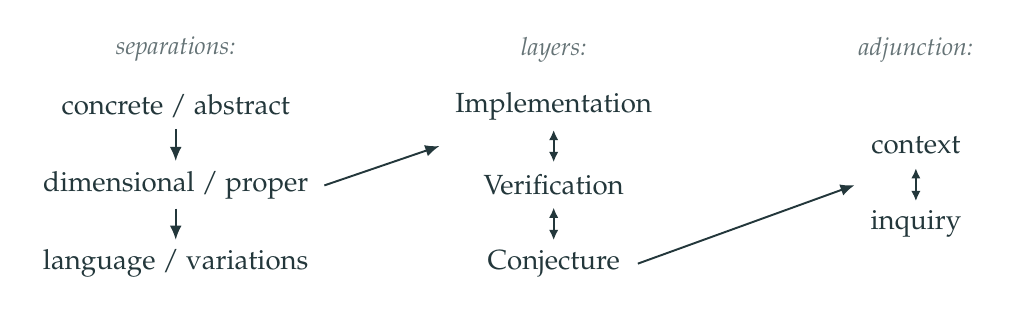
\begin{tikzpicture}[
      every node/.style={align=center, text=presentationgreen},
      layer/.style={minimum height=1.6em},
      columntitle/.style={font=\small\itshape, text=presentationgreen!70},
      arrow/.style={-{Latex[length=1.8mm, width=1.5mm]}, line width=0.7pt, presentationgreen},
      twoway/.style={{Latex[length=1.3mm, width=1.2mm]}-{Latex[length=1.3mm, width=1.2mm]}, line width=0.7pt, presentationgreen},
    ]
    \node[columntitle] at (-4.8, 0.72) {separations:};
    \node[columntitle] at (0, 0.72) {layers:};
    \node[columntitle] at (4.6, 0.72) {adjunction:};

    \node[layer] (implementation) at (0, 0) {Implementation};
    \node[layer] (verification) at (0, -1.0) {Verification};
    \node[layer] (conjecture) at (0, -2.0) {Conjecture};
    \draw[twoway] (implementation) -- coordinate (implementationtoverification) (verification);
    \draw[twoway] (verification) -- (conjecture);
    \node[fit=(implementation) (verification) (conjecture), inner sep=2pt] (layers) {};

    \node[layer] (concreteabstract) at (-4.8, 0) {concrete / abstract};
    \node[layer] (dimensionalproper) at (-4.8, -1.0) {dimensional / proper};
    \node[layer] (languagevariations) at (-4.8, -2.0) {language / variations};
    \draw[arrow] (concreteabstract) -- (dimensionalproper);
    \draw[arrow] (dimensionalproper) -- (languagevariations);
    \node[fit=(concreteabstract) (dimensionalproper) (languagevariations), inner sep=2pt] (separations) {};
    \draw[arrow] (separations.east) -- (layers.west |- implementationtoverification);

    \node[layer] (context) at (4.6, -0.5) {context};
    \node[layer] (inquiry) at (4.6, -1.5) {inquiry};
    \draw[twoway] (context) -- (inquiry);
    \node[fit=(context) (inquiry), inner sep=2pt] (poles) {};
    \draw[arrow] ([xshift=3pt]conjecture.east) -- (poles.west);
  \end{tikzpicture}%
}

% Process, first click: the conversations (C) form a graph T, joined by what passes
% between them (together); verification, the long bent arrow on the right, carries
% T to an exact replica G, the knowledge graph. Nodes, edges and letters take the
% colours of the marked words they stand for.
\newcommand{\processdiagram}{%
  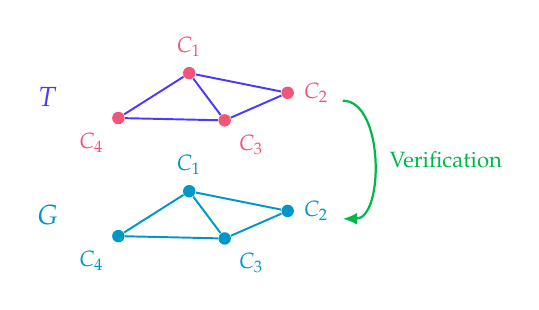
\begin{tikzpicture}[
      conversation/.style={circle, fill=conversationrose, inner sep=0pt, minimum size=4.5pt},
      concept/.style={circle, fill=graphblue, inner sep=0pt, minimum size=4.5pt},
      conversationname/.style={font=\footnotesize, text=conversationrose},
      conceptname/.style={font=\footnotesize, text=graphblue},
      message/.style={messageindigo, line width=0.7pt},
      link/.style={graphblue, line width=0.7pt},
    ]
    \node[conversation, label={[conversationname]above:$C_1$}] (t1) at (0, 0.6) {};
    \node[conversation, label={[conversationname]right:$C_2$}] (t2) at (1.25, 0.35) {};
    \node[conversation, label={[conversationname]below right:$C_3$}] (t3) at (0.45, 0) {};
    \node[conversation, label={[conversationname]below left:$C_4$}] (t4) at (-0.9, 0.03) {};
    \draw[message] (t1) -- (t4)  (t1) -- (t2)  (t1) -- (t3)  (t2) -- (t3)  (t4) -- (t3);
    \node[text=messageindigo] (togethergraph) at (-1.8, 0.3) {$T$};

    \begin{scope}[yshift=-1.5cm]
      \node[concept, label={[conceptname]above:$C_1$}] (g1) at (0, 0.6) {};
      \node[concept, label={[conceptname]right:$C_2$}] (g2) at (1.25, 0.35) {};
      \node[concept, label={[conceptname]below right:$C_3$}] (g3) at (0.45, 0) {};
      \node[concept, label={[conceptname]below left:$C_4$}] (g4) at (-0.9, 0.03) {};
      \draw[link] (g1) -- (g4)  (g1) -- (g2)  (g1) -- (g3)  (g2) -- (g3)  (g4) -- (g3);
      \node[text=graphblue] (knowledgegraph) at (-1.8, 0.3) {$G$};
    \end{scope}

    % Right of both graphs, clear of the C_2 labels: low looseness keeps the bend
    % long and narrow rather than round.
    \draw[-{Latex[length=1.8mm, width=1.5mm]}, verificationgreen, line width=0.8pt]
      (1.95, 0.25) to[out=0, in=0, looseness=0.9]
      node[right, xshift=2pt, font=\footnotesize, text=verificationgreen] {Verification}
      (1.95, -1.25);
  \end{tikzpicture}%
}

% Where we are in the talk: four blocks across the full page width, one per
% section, with the current one filled. The slide number sits directly above them
% in the right corner. A new section starts with \startsection{n}, which moves the
% filled block and switches the title bar and paragraph rules to that section's shade.
% Each block is also a link to the first slide of its section, the frame labelled
% talksection<n>. \talksectionsbuilt counts the sections that exist so far, so the
% footer never links to a missing slide; raise it when a new section starts.
\newcommand{\currenttalkpart}{1}
\newcommand{\startsection}[1]{%
  \renewcommand{\currenttalkpart}{#1}%
  \colorlet{currentsectionshade}{sectionshade#1}%
  \setbeamercolor{frametitle}{bg=sectionshade#1}%
}
\newcommand{\talksectionsbuilt}{4}
\newcommand{\footerblock}[1]{%
  \ifnum#1=\currenttalkpart\relax
    \def\talkpartfill{sectionshade#1}%
  \else
    \def\talkpartfill{none}%
  \fi
  \begin{tikzpicture}[x=0.25\paperwidth, y=5pt]
    \useasboundingbox (0, 0) rectangle (1, 1);
    \draw[sectionshade#1, line width=0.3pt, fill=\talkpartfill] (0, 0) rectangle (1, 1);
  \end{tikzpicture}%
}
\newcommand{\linkedfooterblock}[1]{%
  \ifnum#1>\talksectionsbuilt\relax
    \footerblock{#1}%
  \else
    \hyperlink{talksection#1}{\footerblock{#1}}%
  \fi
}
\newcommand{\footerblocks}{%
  \hbox to \paperwidth{%
    \linkedfooterblock{1}\linkedfooterblock{2}\linkedfooterblock{3}\linkedfooterblock{4}%
  }%
}
\setbeamertemplate{footline}{%
  \vbox{%
    \hbox to \paperwidth{%
      \hfill
      \usebeamerfont{page number in head/foot}%
      \usebeamercolor[fg]{page number in head/foot}%
      \usebeamertemplate*{page number in head/foot}%
      \hspace{1.4em}%
    }%
    \vskip 2pt
    \footerblocks
  }%
}

\title{Hoapa}
\subtitle{Logic, collective inquiry and open-science workshops}
% The name is the title slide's one marked word: on the first click it turns italic,
% in the text colour, and its line follows after a colon on the same line. The empty
% line below keeps the place and date at their current, lower position.
\author[Jean-Charles Belouard]{%
  \alt<2->{\textit{Jean-Charles Belouard}: great engineer, ok driver}{Jean-Charles Belouard}%
  \\[0.8em]\strut
}
% Keep the overlay code out of the PDF's author field.
\hypersetup{pdfauthor={Jean-Charles Belouard}}
\date{Helsinki Logic Group, 11 November 2026}

\begin{document}

% The title slide carries the clickable footer too, but no slide number and no
% filled block: it comes before the first section.
{
  \renewcommand{\currenttalkpart}{0}
  \setbeamertemplate{footline}{\vbox{\footerblocks}}
  \begin{frame}[noframenumbering]
    \titlepage
  \end{frame}
}

\begin{frame}[t,label=talksection1]{Introduction — The context}
  \paragraphtitle{Pitch}
  The core of my research consists in drawing inspiration from the philosophy of mathematics and the engineering of networks to formulate \only<2->{\textcolor{hoapaviolet}{[}}\textcolor<2->{hoapaviolet}{a theory of work constrained by \revealedwordwithpunctuation<3->{permaculturegreen}{``}{permacultural}{''}\\ logic: how to produce reusable results while preserving the conditions for future work}\only<2->{\textcolor{hoapaviolet}{]}}. Applied to collectives, it becomes an extension of the \revealedword<4->{scienceblue}{scientific method} which incorporates participatory democracy and sustainability.

  \medskip
  % The last click replaces the marked words' lines with the small diagram.
  \begin{onlyenv}<1-5>
  \begin{itemize}
    \item<2-> \textcolor{hoapaviolet}{[…]}: one point of view among many
    \item<3-> \markedword{permaculturegreen}{Permacultural}: abstracted into ``concretely minimal, abstractly demanding''
    \item<4-> \markedword{scienceblue}{Scientific method}: \\
      well-regulated scientist–Nature relation + (ad hoc peer review $\hookrightarrow$ universities $\hookrightarrow$ economy) \\
      % The line wraps; a top-aligned box keeps its continuation clear of the arrow.
      $\to$~\begin{minipage}[t]{\dimexpr\linewidth-1.6em\relax}\raggedright
        \revealedword<5->{regulationorange}{well-regulated} network of relations among scientists, each retaining a well-regulated relation with Nature
      \end{minipage}
  \end{itemize}

  % The properties the network's layers secure, centred under the list with a
  % little space above.
  \vspace{4pt}
  \uncover<5->{\par\centering\textcolor{regulationorange}{\texttt{[ perspectivism, decentralization, autonomy, openness to peers, expressiveness, transparency, scalability, self-reflection… ]}}\par}
  \end{onlyenv}
  \begin{onlyenv}<6>
    \begin{center}\pitchdiagram\end{center}
  \end{onlyenv}
\end{frame}

\begin{frame}[t]{Introduction — The context}
  \paragraphtitle{Sources}
  The authors it draws on are mathematicians (F.W. Lawvere, \revealedwordwithpunctuation<2->{risingseateal}{}{A. Grothendieck}{),} philosophers (C.S. Peirce, G. Simondon, G. Deleuze), and \revealedword<4->{scienceblue}{scientists} (S. Kauffman, J. Bowlby). In my project, these approaches meet in \revealedwordwithpunctuation<3->{metaphysicsamber}{}{Albert Lautman}{’s} philosophy of mathematics, as read by Fernando Zalamea (who has been supporting my work).

  \medskip
  \begin{itemize}
    \item<2-> \markedword{risingseateal}{A. Grothendieck}: gives a rich notion of creativity, the relative point of view, naturalness via the rising sea method, ecological thinking… the structure and destination of the project…
    \item<3-> \markedword{metaphysicsamber}{Albert Lautman}: or metaphysics as ``problems the universe was going to run into no matter what'', mathematics and physics as ``effective theories answering those problems''…
    \item<4-> \markedword{scienceblue}{Scientists}: because we're interested in each step of the evolution of the universe, from field theories to origins of life and attachment…
  \end{itemize}

  \uncover<5->{%
    \begin{center}
      \textcolor{hoapaviolet}{…Hoapa as an invariant in the effective theories we see}
    \end{center}%
  }
\end{frame}

\begin{frame}[t]{Introduction — The main thesis}
  \paragraphtitle{Thesis}
  My main thesis states that in a system that puts the dialectic between concrete and abstract to \revealedword<2->{energyorange}{work} (brain, computer, community), the relation between concrete substrate and logical labor must be a resource entirely \revealedword<3->{dedicationmagenta}{dedicated} to the design and application of representations and algorithms. A form of separation between two kinds of \revealedwordwithpunctuation<4->{decompositionocean}{}{decomposition}{—}analytic (as in prime factorization) and synthetic (as in vector coordinates relative to a basis)—is a guiding principle, informed by Lautman, which can keep this relation fruitful: in a community, between thinkers and the knowledge they produce.

  \medskip
  % After the three marked words, Lautman's distinction itself takes the list's place.
  \begin{onlyenv}<1-4>
  \begin{itemize}
    \item<2-> \markedword{energyorange}{Work}: \begin{tabular}[t]{@{}l@{}}
        explosion vs.\ engine, the role of constraints; \\
        engine vs.\ organism, the role of closure; \\
        engine vs.\ computer, the role of the ``abstract loop''
      \end{tabular}%
      \hfill
      \begin{tabular}[t]{@{}r@{}}
        \\
        \footnotesize\textcolor{presentationgreen!70}{(Stuart Kauffman,} \\
        \footnotesize\textcolor{presentationgreen!70}{``Beyond Physics'' talk)}
      \end{tabular}
    \item<3-> \markedword{dedicationmagenta}{Dedicated}: as in computers, in cells, in brains, in communities
    \item<4-> \markedword{decompositionocean}{Decomposition (Lautmanian)}: synthetic (dimensional) $\longleftrightarrow$ analytic (proper)
  \end{itemize}
  \end{onlyenv}
  \begin{onlyenv}<5->
    \begin{center}
      \begin{minipage}{0.9\textwidth}\small
        ``The decomposition of a mathematical entity can be envisaged from two very different points of view: sometimes the decomposition brings to light the particular properties of an entity within the set to which it belongs, and it is characterized by the specificity of its very structure; sometimes on the contrary the decomposition of the entities of the same set is done according to a plan common to them all and thus reflects not only their particular properties, but also their belonging to the same set whose global structure is reflected in that of its elements.''

        \smallskip
        \hfill{\footnotesize\color{presentationgreen!70}A.~Lautman, \textit{Mathematics, Ideas and the Physical Real}, trans.\ S.~B.~Duffy}
      \end{minipage}
    \end{center}
  \end{onlyenv}
\end{frame}

\begin{frame}[t]{Introduction — The main thesis}
  \paragraphtitle{Theory of work}
  The physical starting point is that work depends on \revealedword<2->{constraintred}{constraints} that channel energy into particular effects. In living systems, activity also helps \revealedword<3->{permaculturegreen}{maintain} the machinery that makes further activity possible. \revealedword<4->{abstractmirrorblue}{Abstract} representations and algorithms enable a system to retain and share experience, discover relations, construct and test possibilities, revise its own means of understanding and action, and turn results into conditions for further work. This makes the relation between concrete conditions and abstract operations a powerful resource. Lautman supplies a way to investigate such relations through the mathematical and physical constructions that give them substance; Peirce, Simondon, and Kauffman help connect the question to living beings, their environments, and their practices of understanding. Hoapa's proposed separation between thinkers and the organization of knowledge is an engineering approach to developing this potential.

  \begin{center}
    \uncover<2->{\markedword{constraintred}{Constraints}: effects}
    \uncover<3->{— \markedword{permaculturegreen}{Maintain}: closure}
    \uncover<4->{— \markedword{abstractmirrorblue}{Abstract}: secondary loop}
  \end{center}
\end{frame}

\begin{frame}[t]{Introduction — How Hoapa works}
  \paragraphtitle{Process}
  Hoapa is designed as a network of small \revealedword<2->{conversationrose}{conversations} in which one group's work becomes another group's starting point. A question brings participants \revealedwordwithpunctuation<2->{messageindigo}{}{together}{;} their discussion produces a document that others can examine, challenge, or develop. These documents form a growing map of questions, concepts, arguments, and dependencies: a knowledge \revealedwordwithpunctuation<2->{graphblue}{}{graph}{.} So that contributions can differ and come unforced, the system gives participants control and equal standing (they all play by the same rules they themselves manage). Knowledge acquires structure \revealedword<6->{independencecopper}{independently} of the structure of its producers, be it social, political, economic…

  \medskip
  % Click 2: the three marked words, and the small diagram where their lines will
  % go (drawn as an overlay, so the words stay in place when it leaves). Then one
  % line per click.
  \begin{itemize}
    \item<2-> \markedword{conversationrose}{Conversation}:\only<2>{\tikz[overlay, baseline=0pt]\node[anchor=north west, inner sep=0pt] at (2.7cm, 1.2em) {\processdiagram};} \only<3->{modeled after citizen assemblies (helps autonomy, role-symmetry, modularity… control and equal standing)}
    \item<2-> \markedword{messageindigo}{Together (concurrency)}: \only<4->{message passing style, as in the actor model or $\pi$-calculus}
    \item<2-> \markedword{graphblue}{Graph}: \only<5->{typed knowledge graphs, which are versioned, multiplex, homotopical, federated…}
    \item<6-> \markedword{independencecopper}{Independently}: respecting the concrete/abstract separation of concerns and dedicated relation between the two
  \end{itemize}
\end{frame}

% A first look at the overview diagram, before verification and the conjecture:
% the partial version, which part 3 opens with again before adding the rest.
\begin{frame}[c]{Introduction — How Hoapa works}
  \centering
  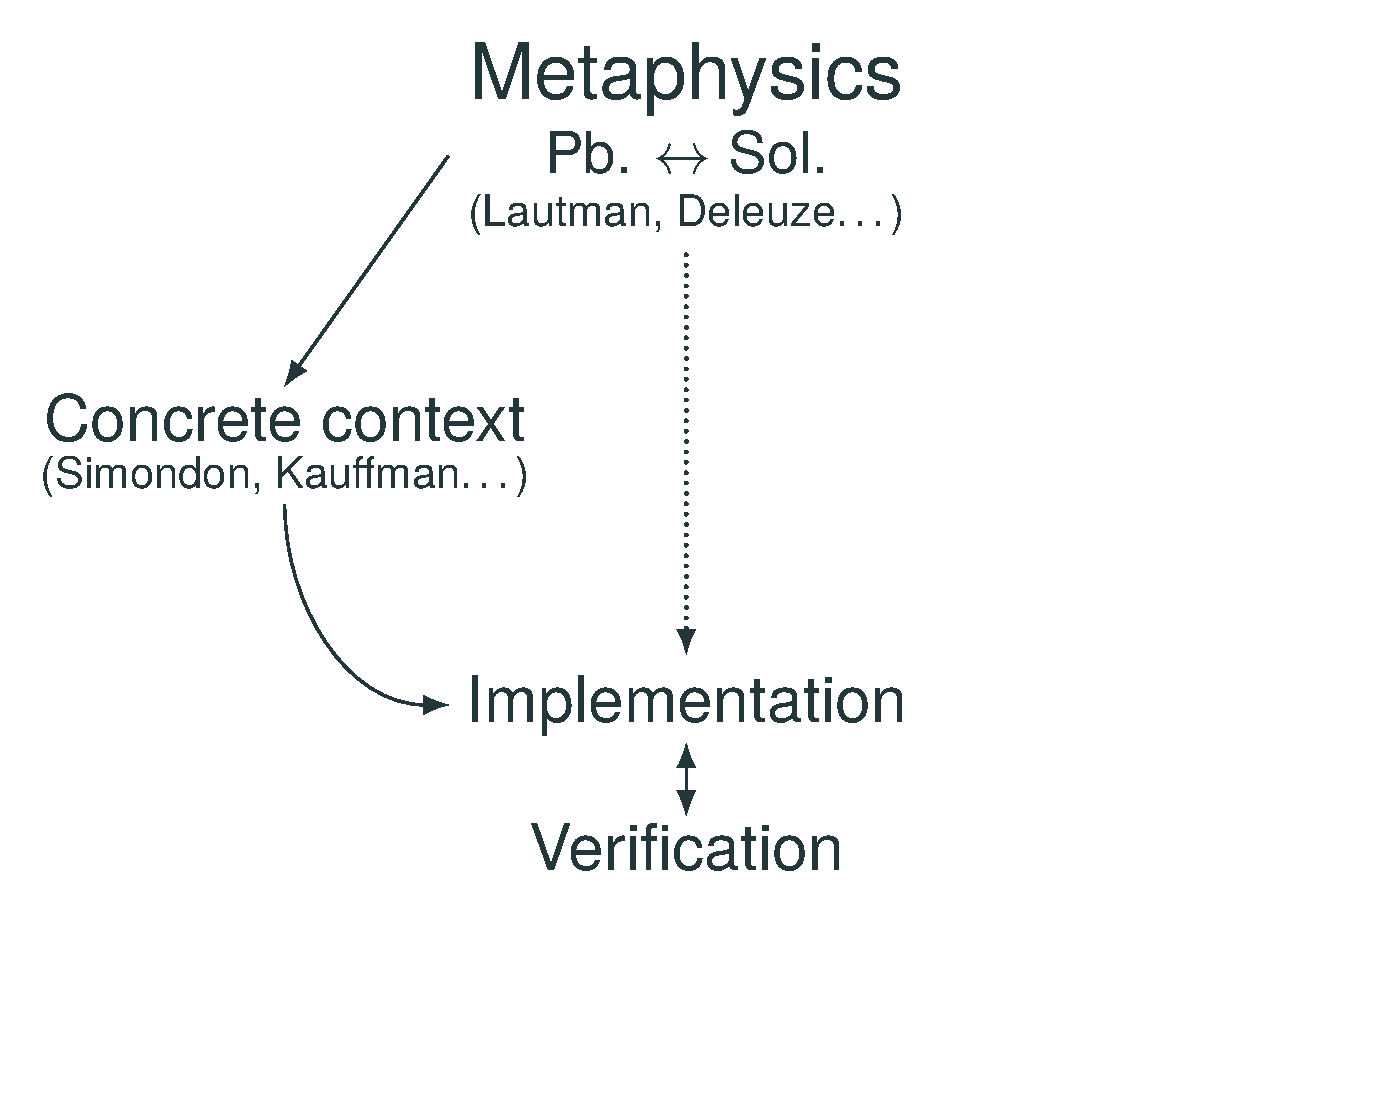
\includegraphics[height=0.85\textheight]{talk_hlg_111126_diagram_partial.pdf}%
\end{frame}

\begin{frame}[t]{Introduction — What is checked, what is conjectured}
  \paragraphtitle{Verification}
  The communication protocols specify how these conversations proceed and how their results enter the shared documentation. Software is used as a \revealedword<2->{refereeyellow}{referee} and is itself subject to modification by the conversations. Alongside the conversation process, a mathematical \revealedword<3->{verificationgreen}{verification} layer is being developed in cubical Agda, a language in which proofs can be checked by a computer. One existing result establishes that consistently renaming \revealedword<4->{participantsplum}{participants} cannot change the checker's verdict. The broader aim is to make the system's promises precise enough to test and prove.

  \medskip
  \begin{itemize}
    \item<2-> \markedword{refereeyellow}{Referee}: or automation as \textit{liberation from control mechanisms}, from the necessity to have management
    \item<3-> \markedword{verificationgreen}{Verification}: machine-checks that the record of each conversation is well-formed according to the protocol, never that its conclusions are true
    \item<4-> \markedword{participantsplum}{Participants}: the protocol is blind to identity of contributors, which means it can't count on specialization (…is knowledge lost?)
  \end{itemize}
\end{frame}

\begin{frame}[t]{Introduction — What is checked, what is conjectured}
  \paragraphtitle{Conjecture}
  The project seeks a mathematical correspondence—an \revealedwordwithpunctuation<2->{adjunctioncrimson}{}{adjunction}{—}\allowbreak between two poles. One organizes inquiry through conversations, verification, and knowledge graphs. The other represents mathematical contexts and the different perspectives through which they can be investigated. The conjecture is guided by an intuition prompted by the perspectival nature of the world: our different understandings of it invite discussion, without presuppositions, from which something the world can reuse may \revealedwordwithpunctuation<3->{emergencecoral}{}{emerge}{.} The conjecture asks whether a \revealedword<4->{universalpropertyblue}{universal property} can distinguish Hoapa’s organization from alternatives. This talk will explore a candidate in which methods are represented by logics and mathematical worlds by the inner models they generate.

  \medskip
  \begin{itemize}
    \item<2-> \markedword{adjunctioncrimson}{Adjunction}: context \& inquiry, perspectivism \& praxis, structure \& genesis/recursion…
    \item<3-> \markedword{emergencecoral}{Emerge}: points to the recursive nature of evolution: physics to biology, biology to psychology…
    \item<4-> \markedword{universalpropertyblue}{Universal property}: ``specialness'' in mathematics $\to$ optimality in engineering
  \end{itemize}
\end{frame}

% The rising sea in Deligne's words: the first 72 seconds of his 1996 lecture in
% Nice, with English subtitles in the picture. The still (at 14 s) shows until the
% video is clicked. Both files sit next to this one: deligne_rising_sea.mp4 and
% deligne_rising_sea_poster.jpg, cut from the full lecture recording.
\begin{frame}[t]{Introduction — From logic to practice}
  \paragraphtitle{Rising sea as a reason to believe in permacultural logic}
  \centering
  \movie[width=0.6\textwidth, height=0.348\textwidth, poster]{%
    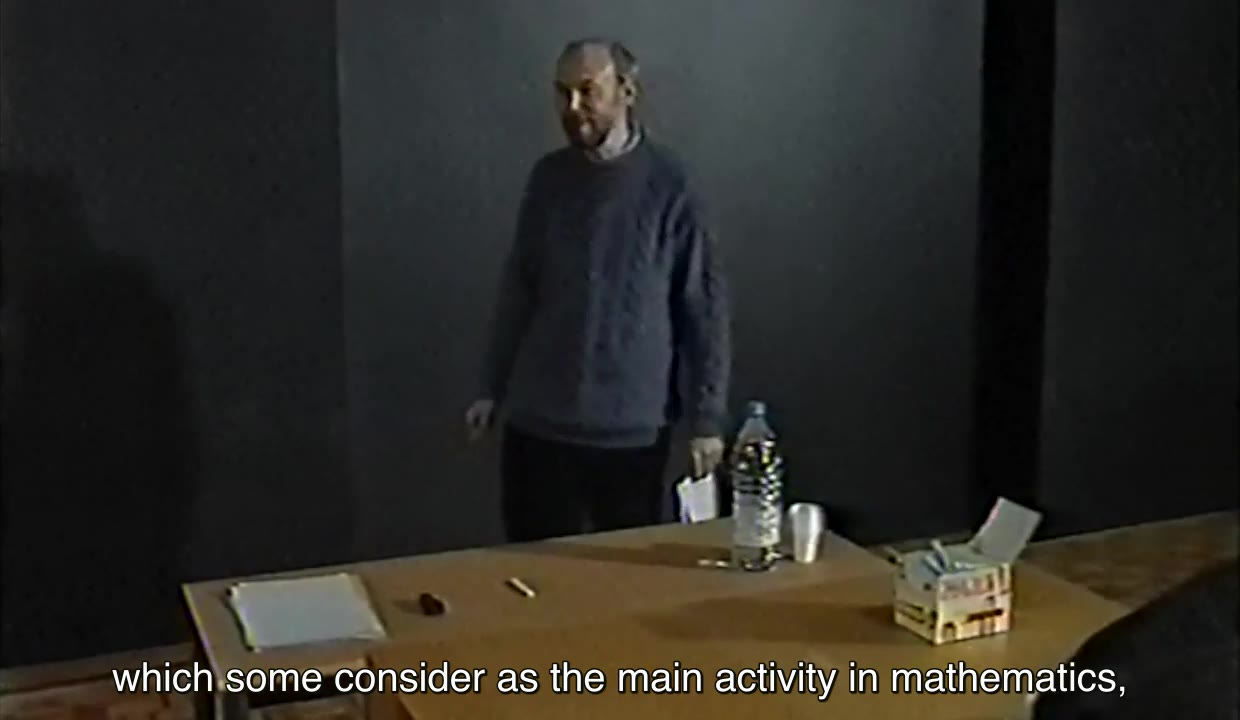
\includegraphics[width=0.6\textwidth, height=0.348\textwidth]{deligne_rising_sea_poster.jpg}%
  }{deligne_rising_sea.mp4}

  \vspace{4pt}
  {\footnotesize\color{presentationgreen!70}P.~Deligne, \textit{L'œuvre d'Alexandre Grothendieck}, Nice, 1996}
\end{frame}

\begin{frame}[t]{Introduction — From logic to practice}
  \paragraphtitle{Permacultural logic}
  The project also looks for this pattern inside logic, where ``permaculture'' is understood broadly as the two-step process of (1) getting to know one's context as much as possible, (2) acting minimally in a manner that will enhance one's condition while preserving and enriching the context. A proof may begin with a provisional assumption (borrow), derive a conclusion (work), and turn the derivation into a conditional statement that later proofs can use (return) or start afresh from \revealedwordwithpunctuation<3->{replayolive}{(}{replay}{).} Hoapa investigates this borrow–work–replay pattern as a possible logical expression of its permacultural ambition: the \revealedword<2->{harmonyorchid}{harmony} between receiving and giving back.

  \medskip
  \begin{itemize}
    \item<2-> \markedword{harmonyorchid}{Harmony}: as in Gentzen, type theory, Hilbert's axiomatic method
    \item<3-> \markedword{replayolive}{Replay}: the hidden part of logic that makes logic work
  \end{itemize}
\end{frame}

\begin{frame}[t]{Introduction — From logic to practice}
  \paragraphtitle{Development}
  The architecture of a ``mature'' Hoapa system is both demanding—to respect its constraints—and—by virtue of presuppositionlessness—\allowbreak\revealedwordwithpunctuation<2->{unpredictablecyan}{}{unpredictable}{.} Autonomous open-science workshops could make these ideas tangible and seed larger systems, embracing both pragmaticism and experimentalism. Their first requirement is usefulness: knowledge sharing must be truly at \revealedwordwithpunctuation<3->{stakebrown}{}{stake}{,} so that the organization develops through serving a real purpose. Concretely, I envision something based on the philosophy of ``document-driven-development'', where \revealedword<4->{documentationink}{documentation} gradually replaces the instructor, both as the joint source of truth and the manager of the process.

  \medskip
  \begin{itemize}
    \item<2-> \markedword{unpredictablecyan}{Unpredictable}: collective inquiry helps determine how collective inquiry is organized
    \item<3-> \markedword{stakebrown}{Stake}: what distinguishes and makes citizen assemblies efficient; you can't simulate life or understanding
    \item<4-> \markedword{documentationink}{Documentation}: does in the Lautmanian-analytic what specialization does in the synthetic agents: shared source and management, but ``softer''
  \end{itemize}
\end{frame}

% Implementation: use cases. Each small paragraph is its own click; a marked word
% takes one more click and shows its line right after its paragraph.
\startsection{2}

\begin{frame}[t,label=talksection2]{Implementation — Use cases}
  \paragraphtitle{A park}
  \balancedstart
  Hoapa can also operate at small scales and with only the ``base layer of complexity'' which separates the role-symmetric agents from the typed documentation they produce.

  \begin{uncoverenv}<2->
    For instance we could have a neighborhood ``manage'' its local park via a protocol in which the motivated residents discuss how it could be enhanced, and produce a to-do list for its maintenance.
  \end{uncoverenv}

  \begin{uncoverenv}<3->
    Here it is crucial to understand that the system can preserve its advantageous mathematical, social and engineering properties if it is \textbf{only} a communication system, and not a full management system which also enacts in reality what has been discussed in the abstract.
  \end{uncoverenv}
\end{frame}

\begin{frame}[t]{Implementation — Use cases}
  \paragraphtitle{A park}
  \balancedstart
  Its task is to chart the world and design appropriate algorithms, not interfere with and certainly not control it. (That would kill all the carefully crafted separations of concerns, starting with the role-symmetry of agents, because it necessarily introduces some hierarchical structure and tension—for basically the same reasons you can share an idea with the entire world without losing it, but you can't do that with a loaf of bread.)\end{frame}

\begin{frame}[t]{Implementation — Use cases}
  \paragraphtitle{A park}
  \balancedstart
  Hoapa protocols can interact with the world only behind buffers which respect individual freedom:

  \begin{itemize}
    \item<2-> If it needs something it simply asks for it, and expects those needs to be met (for instance, if it uses the internet, it states via a self-reflective conversation how much bandwidth it needs, and specifies the characteristics of its network). Individuals or communities, outside of the protocol, would then respond to those needs without compensation.
    \item<3-> If it wants something to be known it simply makes it as available and accessible as possible, which includes a pedagogical effort in presentation and terminology. But it can't advertise, at the risk of favoring certain targets over others.
  \end{itemize}

  \begin{uncoverenv}<4->
    In either direction, we can think of Hoapa as a coach in sports: its domain of action is preparation and strategy, but it can never enter the field of play or control the players. The game belongs to the players.
  \end{uncoverenv}
\end{frame}

\begin{frame}[t]{Implementation — Use cases}
  \paragraphtitle{A park}
  \balancedstart
  In this example, we can imagine an institution/Hoapa hybrid in which the city government has delegated the supervision of the park to the protocol, but it's still the paid workforce of gardeners which will perform the tasks suggested by the protocol. But ideally, in the spirit of the protocol, it would be only voluntary work, suggested by the protocol but decided at the level of the individuals and communities.

  \begin{uncoverenv}<2->
    \transitionsentence{Which makes Hoapa protocols especially well suited to organize the open source economy.}
  \end{uncoverenv}
\end{frame}

\begin{frame}[t]{Implementation — Use cases}
  \paragraphtitle{Open source}
  \balancedstart
  Because open source produces code, it mostly ``lives in the abstract''. Historically, it has also used a lot of voluntary labor. So it is by design a process that respects the separation of concerns Hoapa systems start with.

  \begin{uncoverenv}<2->
    The main recurring problem open source projects face is scalability and continuation beyond the circle of core contributors and maintainers, usually the instigators of the project: because open source projects are structured around ``circles of knowledge and influence'', which is in essence a hierarchy, it is very likely to terminate the moment the inner circle quits.
  \end{uncoverenv}
\end{frame}

\begin{frame}[t]{Implementation — Use cases}
  \paragraphtitle{Open source}
  \balancedstart
  Hoapa revokes the privileges of the inner circle, distributes the workload evenly and transfers all the essential knowledge from the original designer's minds into a strictly typed and \revealedwordwithpunctuation<2->{documentationink}{}{operational documentation}{.}

  \begin{itemize}
    \item<2-> \markedword{documentationink}{Operational documentation}: for instance, using team semantics and provenance, what must remain traceable for others to understand, revise, and continue the work (as an extension to the collective of Knuth's literate programming)
  \end{itemize}

  \begin{uncoverenv}<3->
    While this is more demanding in the early stages of the process, it pays off by making the project truly scalable and persistent (not persistent in the sense of a capitalistic endeavor, which always needs to grow and colonize new markets, but closer to how ecosystems work, with minimalism and circularity).
  \end{uncoverenv}

  \begin{uncoverenv}<4->
    \transitionsentence{The same arguments can be used to suggest a reform of how science is conducted.}
  \end{uncoverenv}
\end{frame}

\begin{frame}[t]{Implementation — Use cases}
  \paragraphtitle{Science}
  \balancedstart
  \alt<2->{\sout{Universities organize inquiry through hierarchies that also distribute funding, employment, and recognition. These dependencies influence which questions can be pursued and whose contributions are heard.}}{Universities organize inquiry through hierarchies that also distribute funding, employment, and recognition. These dependencies influence which questions can be pursued and whose contributions are heard.}

  \begin{uncoverenv}<2->
    Universities are extremely hierarchical political machines whose ties to reality are clearly not behind buffers, which impair their capacity to describe the world they inhabit.*
  \end{uncoverenv}

  \begin{uncoverenv}<3->
    While the scientific method, in the domains where it is applicable, makes claims answerable to evidence and correction, it doesn't prevent other types of evils. Notably a mismanagement of efforts toward certain technologies at the expense of understanding, the fragmentation of the study of Nature into opposing departments, the proliferation of opaque jargons, the insistence that there exists a ``view from nowhere'', the enclosure of knowledge behind paywalls, proprietary tools, and restricted access, the depreciation of errors and failures, etc.
  \end{uncoverenv}

\end{frame}

\begin{frame}[t]{Implementation — Use cases}
  \paragraphtitle{Science}
  \balancedstart
  Hoapa protocols, on the other hand, are ideal for the realization of what citizen science promised to be, but only marginally developed. In a real and, hopefully, demonstrable sense, they are an extension of the Galilean scientific method to the collective.

  \begin{uncoverenv}<2->
    In the Hoapa extension, we define how scientists are supposed to converse among themselves, and how they should refine and store information into a strictly typed and operational technical \revealedwordwithpunctuation<3->{languageamethyst}{}{language}{.} Our conjecture is that a universal property can distinguish Hoapa among organizations pursuing this work.
  \end{uncoverenv}

  \begin{itemize}
    \item<3-> \markedword{languageamethyst}{Language}: ``Learn once, write everywhere'' $\leftarrow$ a shared conceptual landscape built through explicit and systematic comparisons (interpretation, equivalence, coherence…)
  \end{itemize}
\end{frame}

\begin{frame}[t]{Implementation — Use cases}
  \paragraphtitle{Science}
  \balancedstart
  Hoapa protocols are designed for education, as part of their mandate to treat everybody on an equal footing. What is removed with the status is not the knowledge, but the hunt for the status, and at the same time it resituates the obligation to make one's specialized knowledge accessible to others.

  \begin{uncoverenv}<2->
    Crucially, each individual practitioner gets to decide what questions are worth pursuing, opening a path to restoring science’s sense of purpose from the ground up.
  \end{uncoverenv}

  \begin{uncoverenv}<3->
    \transitionsentence{And the organization of inquiry is itself something we can try to understand mathematically.}
  \end{uncoverenv}
\end{frame}

\begin{frame}[t]{Implementation — Use cases}
  \paragraphtitle{Mathematics}
  \balancedstart
  All of the above applies in mathematics as well, but here the connection goes \revealedwordwithpunctuation<3->{emergencecoral}{}{further}{:} mathematics also supplies the language in which the organization of mathematical work can itself be investigated. Hoapa’s formalization uses Cubical Agda, bringing together homotopy type theory, computer-checked proofs, and a line of thought connecting Alexander Grothendieck’s ideas about homotopy types and higher groupoids with Vladimir Voevodsky’s univalent foundations.

  \begin{uncoverenv}<2->
    Hoapa proposes to carry this connection into the organization of collective inquiry itself. This ambition echoes Grothendieck’s memoirs, which weave together reflections on creativity, mathematical practice and mathematics itself.
  \end{uncoverenv}

  % Exceptionally, the transition sentence replaces the marked word's line on the
  % next click: the slide has no room for both. overprint reserves the taller of
  % the two, so nothing above moves. The space before it restores the gap a list
  % would normally leave after a paragraph, which overprint drops.
  \vspace{8pt}
  \begin{overprint}
    \onslide<3>
      \begin{itemize}
        \item \markedword{emergencecoral}{Further}: a method of articulating a context can generate a new context for further inquiry (in math and logic, in generalized evolution)
      \end{itemize}
    \onslide<4->
      \transitionsentence{Grothendieck also questioned the ecological consequences of scientific activity; Hoapa approaches that concern by asking how understanding a world can help us inhabit it.}
  \end{overprint}
\end{frame}

\begin{frame}[t]{Implementation — Use cases}
  \paragraphtitle{Generalized permaculture}
  \balancedstart
  I believe Hoapa protocols can stage and target the kind of recursive and self-reflective patterns just mentioned, in harmony with the ecosystem, by generalizing the concept of permaculture and applying it to a vast majority of human endeavors. Permaculture could in effect become the default mode of being of humanity, following this very simple algorithm:

  \begin{itemize}
    \item<2-> Make a very detailed and executable map of your environment, including your imprint on it.
    \item<3-> Use it to figure out what is best for both you and your environment, and do it (which becomes the default if individual freedom replaces ``investability'' as the condition for action).
  \end{itemize}
\end{frame}

\begin{frame}[t]{Implementation — Use cases}
  \paragraphtitle{Generalized permaculture}
  \balancedstart
  This is where the ``layers of complexity'' which respect and target perspectivism, decentralization, autonomy, openness to peers, expressiveness, transparency, scalability and self-reflection, start to be really useful.

  \begin{uncoverenv}<2->
    \transitionsentence{To tend a place is also to attend to the relations that sustain it—and those relations lead us into a network.}
  \end{uncoverenv}
\end{frame}

\begin{frame}[t]{Implementation — Use cases}
  \paragraphtitle{Networks}
  \balancedstart
  In all the preceding examples we've looked at instances of Hoapa protocols in isolation, but each of them would be better envisioned as a node of a vast network.

  \begin{uncoverenv}<2->
    A mature protocol regulating a park would necessarily have typed conversations with other park protocols, especially those close by, to share information and reuse each other's research. It would also have ties to all the independent protocols a city would be made up of: electricity grid, water management, transportation, agriculture… and then beyond the city limits, into all sorts of other communities organized through protocols, each bringing its own point of view, from playground design to natural philosophy.
  \end{uncoverenv}

  \begin{uncoverenv}<3->
    A park’s investigation of soil and water becomes useful to another park; a software improvement made for its documentation becomes available to other projects; a scientific question raised locally finds research communities elsewhere equipped to pursue it. The park community’s teaching material can help newcomers elsewhere. And communities can help one another translate documentation, test proposals, or investigate disagreements. Records of failed attempts can spare others the same mistakes.
  \end{uncoverenv}
\end{frame}

\begin{frame}[t]{Implementation — Use cases}
  \paragraphtitle{Networks}
  \balancedstart
  In all of this, each protocol is both an agent and a recipient of \revealedwordwithpunctuation<2->{careterracotta}{}{care}{,} as a concrete ecosystem as well as an abstract community of participants.

  \begin{itemize}
    \item<2-> \markedword{careterracotta}{Care}: Hoapa’s generalization of attachment theory (biology, psychology) into a two-step reciprocal and cyclic algorithm
      \begin{enumerate}
        \item<3-> In a given network, the evolution toward maturity of newer elements is taken care of by the mature elements already present in the network
        \item<4-> In turn, those newer elements become mature and take care of a new generation of elements
      \end{enumerate}
  \end{itemize}
\end{frame}

% Part 3: the conjecture. The overview diagram comes in two clicks: what has been
% covered so far, then the full picture. Both PDFs share one canvas (see
% talk_hlg_111126_diagram_full.tex), so the second simply adds to the first.
\startsection{3}

\begin{frame}[c,label=talksection3]{The Hoapa conjecture — an adjunction}
  \centering
  \includegraphics<1>[height=0.85\textheight]{talk_hlg_111126_diagram_partial.pdf}%
  \includegraphics<2>[height=0.85\textheight]{talk_hlg_111126_diagram_full.pdf}%
\end{frame}

\begin{frame}[t]{The Hoapa conjecture — an adjunction}
  \paragraphtitle{Motivations and goals}
  \balancedstart
  To motivate its adoption and distinguish Hoapa from other “interesting projects” we can attach buzzwords to, I need a mathematical reason for organizing inquiry this way. The goal is to characterize Hoapa by a universal property, in a setting that represents both the contexts it investigates and alternative ways of investigating them.

  \begin{uncoverenv}<2->
    If the conjecture succeeds, this universal property would translate into a claim of \revealedword<3->{optimalitygold}{optimality} for any implementation satisfying its conditions. The world we inhabit must explain why those conditions matter. Hoapa is also its own experiment: implementing its protocols lets us test the conjecture's claims.
  \end{uncoverenv}

  \begin{itemize}
    \item<3-> \markedword{optimalitygold}{Optimality}: the constraints imposed on a process, in a given context, to achieve an intended outcome\\
      constraints = the protocol; process = collective inquiry; context = this world;\\
      outcome = understanding that enables generalized permaculture to be enacted
  \end{itemize}
\end{frame}

\begin{frame}[t]{The Hoapa conjecture — an adjunction}
  \paragraphtitle{Motivations and goals}
  \balancedstart
  \revealedfirstword<2->{hoapaviolet}{Perspectivism} motivates this ambition; \revealedword<3->{presuppositionlessnessteal}{presuppositionlessness} guides the response. The world has already produced different beings, experiences, skills, and ways of understanding. Their contributions must be able to enter the inquiry without their worth being decided in advance by a hierarchy or an established division of knowledge. What the world has already developed becomes material for collective work; what that work will produce remains open.

  \begin{itemize}
    \item<2-> \markedword{hoapaviolet}{Perspectivism}: global understanding is assembled from local views, with obstructions to their integration retained as information
    \item<3-> \markedword{presuppositionlessnessteal}{Presuppositionlessness}: applied to protocols, a principle saying we need common rules, open rules with equally distributed power to revise them, and only the rules needed to make communication possible
  \end{itemize}
\end{frame}

\begin{frame}[t]{The Hoapa conjecture — an adjunction}
  \paragraphtitle{Categories from metaphysics}
  \balancedstart
  The proposed adjunction relates a category of contexts to a category of organizations of inquiry: write $\mathbf{Ctx}$ for the first and $\mathbf{Inq}$ for the second. We seek functors $F\colon \mathbf{Ctx}\to\mathbf{Inq}$ and $G\colon \mathbf{Inq}\to\mathbf{Ctx}$ with natural bijections $\mathrm{Hom}_{\mathbf{Inq}}(Fc, i) \cong \mathrm{Hom}_{\mathbf{Ctx}}(c, Gi)$. The unit $\eta_c\colon c\to GFc$ and the counit $\varepsilon_i\colon FGi\to i$ compare each side with its round trip. The mathematical form of $\mathbf{Ctx}$ is still under investigation, and neither functor has been constructed.
\end{frame}

\begin{frame}[t]{The Hoapa conjecture — an adjunction}
  \paragraphtitle{Categories from metaphysics}
  \balancedstart
  Each piece of this structure is meant to carry one of the project's concepts: \revealedwordwithpunctuation<2->{complexityazure}{}{$F$}{,} \revealedwordwithpunctuation<3->{emergencecoral}{}{$G$}{,} the unit \revealedword<4->{praxispurple}{$\eta$} and the counit \revealedwordwithpunctuation<5->{anthropiclosspink}{}{$\varepsilon$}{.}

  \begin{itemize}
    \item<2-> \markedword{complexityazure}{$F$}: Complexity, the organized work a context allows
    \item<3-> \markedword{emergencecoral}{$G$}: Evolution, what organized inquiry produces can become part of the conditions under which further inquiry takes place
    \item<4-> \markedword{praxispurple}{$\eta$}: Praxis, the difference between what a context makes possible and what a particular inquiry actually does with those possibilities
    \item<5-> \markedword{anthropiclosspink}{$\varepsilon$}: Anthropic loss, the possible failure of the reconstruction map $\varepsilon_i\colon FGi\to i$ to be invertible
  \end{itemize}
\end{frame}

% Permacultural logic from the adjunction: still Part 3, so the title bar stays;
% each subsection's title follows "Permacultural logic —" as the paragraph title,
% and each subsection takes two slides. The oral-commentary footnotes in the text
% file stay off the slides. These slides are shown, not presented: each appears
% whole, in one step, for the audience to skim (every overlay starts at <1->).

\begin{frame}[t]{The Hoapa conjecture — an adjunction}
  \paragraphtitle{Permacultural logic — From work to reusable construction}
  \balancedstart
  The permacultural question is how an achievement becomes a means of further construction. Implication provides a precise mathematical example. We borrow an assumption $A$, derive $B$, and \revealedword<1->{returnroyal}{return} the derivation as an implication. Other proofs can \revealedword<1->{replayolive}{replay} that work when its conditions are supplied.

  \begin{itemize}
    \item<1-> \markedword{returnroyal}{Return}: abstraction turns $w\colon \Gamma\times A\to B$ into $w^{\sharp}\colon \Gamma\to A\Rightarrow B$.
    \item<1-> \markedword{replayolive}{Replay}: evaluation applies the returned operation to an input: $(A\Rightarrow B)\times A\to B$.
  \end{itemize}
\end{frame}

\begin{frame}[t]{The Hoapa conjecture — an adjunction}
  \paragraphtitle{Permacultural logic — From work to reusable construction}
  \balancedstart
  In the cartesian closed interpretation of intuitionistic logic, this is the adjunction:
  \[
    (-\times A)\dashv(A\Rightarrow -)
    \qquad
    \mathrm{Hom}(\Gamma\times A, B)\cong\mathrm{Hom}(\Gamma, A\Rightarrow B)
  \]

  \begin{uncoverenv}<1->
    The remaining assumptions $\Gamma$ stay visible: discharging one dependency does not erase the others. Introduction and elimination are governed by \revealedwordwithpunctuation<1->{harmonyorchid}{}{harmony}{.} Their compatibility makes work under an assumption interchangeable with a reusable operation expecting that assumption.
  \end{uncoverenv}

  \begin{itemize}
    \item<1-> \markedword{harmonyorchid}{Harmony}: $\beta$ and $\eta$ make currying and uncurrying inverse—elimination extracts neither more nor less than introduction warrants.
  \end{itemize}
\end{frame}

\begin{frame}[t]{The Hoapa conjecture — an adjunction}
  \paragraphtitle{Permacultural logic — What does the work leave available?}
  \balancedstart
  The same adjunction produces two familiar constructions. The \revealedword<1->{statemonadcerulean}{state monad} composes computations by passing the state left by one into the next. The \revealedword<1->{storecomonadtangerine}{store comonad} holds a family of values together with a selected position, and allows that family to be considered from each position.

  \begin{itemize}
    \item<1-> \markedword{statemonadcerulean}{State monad}: $\mathrm{State}_A(X) = A\Rightarrow(X\times A)$—receive a state; return a result and a resulting state.
    \item<1-> \markedword{storecomonadtangerine}{Store comonad}: $\mathrm{Store}_A(X) = (A\Rightarrow X)\times A$—retain an indexed family and a current position.
  \end{itemize}

  \begin{uncoverenv}<1->
    These structures organize work and access to its setting. Their laws alone do not preserve the conditions for further work. A computation $p(a) = (x, a_0)$ can replace every incoming state with the same $a_0$, erasing distinctions that subsequent work needs.
  \end{uncoverenv}
\end{frame}

\begin{frame}[t]{The Hoapa conjecture — an adjunction}
  \paragraphtitle{Permacultural logic — What does the work leave available?}
  \balancedstart
  Hoapa therefore asks about \revealedwordwithpunctuation<1->{continuationmint}{}{continuation}{:} can the work we intend to do next still be performed from what has been returned? A publication may be sufficient for one use and insufficient for another. The requirement must specify what is to remain possible.

  \begin{itemize}
    \item<1-> \markedword{continuationmint}{Continuation}: $q'\circ w = \bar{w}\circ q$—$q$ and $q'$ publish before and after the work $w$; $\bar{w}$ performs the corresponding operation using only the published input.
  \end{itemize}
\end{frame}

\begin{frame}[t]{The Hoapa conjecture — an adjunction}
  \paragraphtitle{Permacultural logic — The economy of replay}
  \balancedstart
  Earlier I called replay ``the hidden part of logic that makes logic work.'' \revealedword<1->{replayolive}{Cut} gives this phrase a precise sense. An established result enters a later proof; cut elimination can remove that intermediate use without changing what is provable. But removing it can make the proof enormously longer.

  \begin{itemize}
    \item<1-> \markedword{replayolive}{Cut}: a proved result becomes a premise of further reasoning.
  \end{itemize}
\end{frame}

\begin{frame}[t]{The Hoapa conjecture — an adjunction}
  \paragraphtitle{Permacultural logic — The economy of replay}
  \balancedstart
  There are families of short proofs with cut whose shortest cut-free proofs grow beyond every elementary bound in the original proof lengths. Reuse can therefore be dispensable for provability and decisive for \revealedwordwithpunctuation<1->{feasibilitysienna}{}{feasibility}{.}

  \begin{itemize}
    \item<1-> \markedword{feasibilitysienna}{Feasibility}: the same conclusions can require radically different proof lengths; preserving intermediate achievements can make complex work practicable.
  \end{itemize}

  \begin{uncoverenv}<1->
    This gives the sustainability intuition a concrete dimension. Mathematical development concerns what our means of reasoning let us accomplish with finite resources. An achievement can leave the set of consequences unchanged while transforming our capacity to establish and use them.
  \end{uncoverenv}
\end{frame}

\begin{frame}[t]{The Hoapa conjecture — an adjunction}
  \paragraphtitle{Permacultural logic — Achievements become means of inquiry}
  \balancedstart
  A further step occurs when an achievement changes the tools through which inquiry proceeds. In proof by \revealedwordwithpunctuation<1->{reflectionviolet}{}{reflection}{,} a procedure is defined, its correctness is proved, and that proof supports its use in subsequent reasoning. Coq's \texttt{ring} tactic provides a concrete example: established mathematics becomes machinery for later mathematics, while the existing kernel continues to check the proofs.

  \begin{itemize}
    \item<1-> \markedword{reflectionviolet}{Reflection}: a verified procedure becomes part of the proof-producing toolbox, without becoming a new trusted rule.
  \end{itemize}

  \begin{uncoverenv}<1->
    The reusable material can also widen: from derivations in Gentzen's systems, to formalized theories in Hilbert's metamathematics, to constructions and their transport between equivalent types in HoTT. Lautman's passage from structure to genesis, and Simondon's account of produced structures supporting further structuring, guide our interpretation of this movement.
  \end{uncoverenv}
\end{frame}

\begin{frame}[t]{The Hoapa conjecture — an adjunction}
  \paragraphtitle{Permacultural logic — Achievements become means of inquiry}
  \balancedstart
  \revealedfirstword<1->{emergencecoral}{Renewal} occurs when achievements change what further work can do. With Kauffman, we must also ask whether the organization producing them maintains its \revealedwordwithpunctuation<1->{permaculturegreen}{}{conditions of activity}{.} Hoapa's evolutionary hypothesis joins these demands: work should produce reusable achievements while sustaining and developing the conditions for further work.

  \begin{itemize}
    \item<1-> \markedword{emergencecoral}{Renewal}: preserve declared earlier uses and make a genuinely new operation available.
    \item<1-> \markedword{permaculturegreen}{Conditions of activity}: reusable results still depend on people, skills, records, tools, and material support.
  \end{itemize}
\end{frame}

% Part 4: the conclusion, read as written, without commentary. It opens on the
% title alone; the first click brackets it (one conclusion among many); then, as in
% the use cases, each paragraph is its own click. Two slides: the text is too long for
% one at the slides' type size.
\startsection{4}

\begin{frame}[t,label=talksection4]{Conclusion}
  \paragraphtitle{\bracketedtitle<2->{Conclusion}}
  \balancedstart
  \begin{uncoverenv}<3->
    To me, Hoapa is a theory of everywhere: the humble counterpart to a theory of everything.
  \end{uncoverenv}

  \begin{uncoverenv}<4->
    \textit{Hoapa} means ``everywhere'', in the sense of every domain, in Khoekhoegowab, a Khoe language spoken in Namibia, Botswana and South Africa.
  \end{uncoverenv}

  \begin{uncoverenv}<5->
    The egalitarian societies of Africa, such as the San and the Hadza, can be seen as the first human implementers of Hoapa systems.
  \end{uncoverenv}

  \begin{uncoverenv}<6->
    The debate about human nature, a nature Hoapa trusts, turns on how we view the Paleolithic, our deep past: as violent and brutish, or as complex and social. The contrast echoes the one between selection and adaptation.
  \end{uncoverenv}
\end{frame}

\begin{frame}[t]{Conclusion}
  \paragraphtitle{\bracketedtitle<1->{Conclusion}}
  \balancedstart
  Inquiry in universities shows the same structure across many disciplines: two camps, a ``mainstream'' and its ``rebels''. The mainstream reduces Nature's complexity and robs Her of what makes Her trustworthy. (That trust is then quietly transferred to structures of control: hierarchies, capitalism, and ``reason'' as understood from Galton to Dawkins.) The rebels form a holistic camp, which offers a fuller picture, more adequate to understand our own adaptation.

  \begin{uncoverenv}<2->
    Hoapa would give these movements a chance to federate and to find strength in numbers, through a broad base of support in citizen science. Together, they could do justice to the complexity of Nature. We hope this would also bring peace to our relationship with Her and to our relationships with one another, and end the systematic exploitation of Nature and of ourselves.
  \end{uncoverenv}
\end{frame}

\end{document}
